\documentclass[runningheads]{llncs}

\usepackage[T1]{fontenc}
\let\vec\relax
\usepackage{graphicx}
\usepackage{booktabs,multirow,array}
\usepackage{amssymb}
\usepackage{xcolor}
\usepackage[hidelinks,colorlinks=true,
            linkcolor=blue!60!black,
            citecolor=blue!60!black,
            urlcolor=blue!65!black]{hyperref}
\usepackage[numbers,sort&compress]{natbib}
\usepackage[protrusion=false,expansion=false]{microtype}
\usepackage[shortlabels]{enumitem}
\usepackage[section]{placeins}

\graphicspath{{./}{../}}

\emergencystretch=2em
\sloppy

\title{When Graph Structure Becomes a Liability:\\
Temporal Shift in GNN Fraud Detection}

\titlerunning{When Graph Structure Becomes a Liability}

\author{Saket Maganti}
\authorrunning{S. Maganti}

\institute{}

\begin{document}
\maketitle

\begin{abstract}
Graph Neural Networks are assumed to outperform feature-only baselines
on financial fraud detection because transaction networks carry
structural signals absent from individual features.  We test that
assumption under inductive evaluation on the Elliptic Bitcoin Dataset
(203,769 nodes, 234,355 edges, 49 temporal steps) and find the opposite.
A Random Forest achieves F1\,=\,0.820 with no graph structure at all.
A three-layer MLP reaches F1\,=\,0.744\,$\pm$\,0.005 and outperforms
every GNN; GraphSAGE, the best graph model, reaches only
F1\,=\,0.697\,$\pm$\,0.009.  A graph-structure ablation confirms that
the original transaction edges actively harm GNNs: shuffled random
edges improve F1 from 0.268 to 0.383.  The root cause is temporal
distribution shift---the illicit rate drops from 11.6\,\% in training
to 0.3\,\% in the hardest test steps, and all models collapse after
step~42.  Temperature scaling yields $\Delta$F1\,=\,0 and ECE moves
from 0.284 to 0.282, ruling out calibration fixes.  A concat hybrid
(GNN embeddings + raw features fed to Random Forest) recovers to
F1\,=\,0.807, showing graph-derived representations carry complementary
signal only when fused with tabular features.

\keywords{Graph neural networks \and fraud detection \and temporal
distribution shift \and Bitcoin \and concept drift \and
inductive evaluation}
\end{abstract}

\section{Introduction}

Financial fraud on blockchain networks has become a standard application
for Graph Neural Networks~\citep{akoglu2015graph,hilal2022fraud}.
Laundering requires multi-hop layering, fraud rings share wallets, and
mixing services leave topological motifs that isolated features cannot
capture~\citep{meiklejohn2013bitcoin}.

The Elliptic Bitcoin Dataset~\citep{weber2019} has reinforced the view
that GNNs help.  Published results show GCN at
F1\,=\,0.70~\citep{weber2019}, augmented GCN at
0.74~\citep{alarab2020}, GraphSAGE at 0.75~\citep{lo2023}, and
EvolveGCN at 0.77~\citep{pareja2020evolvegcn}.  However, all prior work
uses transductive evaluation (test edges visible during training) and
aggregates over the full test window, hiding per-step degradation.  This
paper enforces inductive evaluation and per-step analysis.  The results
change substantially: a plain MLP beats every GNN, a Random Forest beats
both, and graph structure becomes a measurable liability once the fraud
topology shifts.

Our contributions are:
\begin{itemize}[leftmargin=*,nosep]
\item A three-seed inductive benchmark of GCN, GraphSAGE, GAT, and MLP
  across three class-imbalance strategies, with RF and XGBoost baselines.
\item Per-step temporal analysis exposing model collapse after step~42.
\item A graph-structure ablation proving original edges degrade
  performance below random wiring.
\item A concat hybrid architecture recovering F1\,=\,0.807 by fusing
  GNN embeddings with tabular features.
\item Calibration analysis ruling out post-hoc fixes
  ($\Delta$F1\,=\,0, $\Delta$ECE\,$<$\,0.002).
\end{itemize}

\section{Related Work}

Weber et al.~\citep{weber2019} introduced the Elliptic benchmark with
Random Forest (F1\,=\,0.64), Logistic Regression (F1\,=\,0.53), and GCN
(F1\,=\,0.70).  Subsequent work improved on these numbers through
feature engineering~\citep{alarab2020}, temporal graph
evolution~\citep{pareja2020evolvegcn}, and self-supervised
pre-training~\citep{lo2023}.  All studies use transductive evaluation
and aggregate reporting.

The architectures tested---GCN~\citep{kipf2017},
GraphSAGE~\citep{hamilton2017}, GAT~\citep{velickovic2018}---fall under
the message-passing framework~\citep{gilmer2017mpnn}.  Temporal
extensions~\citep{pareja2020evolvegcn,sankar2020,you2022roland} capture
graph dynamics but require full snapshots.  Class imbalance is typically
addressed via SMOTE~\citep{chawla2002smote} or weighted losses.
Calibration~\citep{guo2017calibration} and concept
drift~\citep{gama2014survey,lu2018drift,quinonero2009shift} are related
concerns; our findings suggest drift is the dominant failure mode here.

\section{Dataset}

The Elliptic Bitcoin Dataset~\citep{weber2019} contains 203,769
transactions (nodes), 234,355 edges, and 165 features per node (94
local transaction features, 71 aggregated neighbourhood features).
Of 46,564 labelled nodes, 4,545 are illicit and 42,019 are licit.
Data spans 49 temporal steps; the standard split trains on steps~1--34
and tests on steps~35--49.

\begin{table}[!htbp]
\centering
\caption{Elliptic dataset summary.}
\label{tab:dataset}
\small
\begin{tabular}{lr}
\toprule
\textbf{Property} & \textbf{Value} \\
\midrule
Nodes & 203,769 \\
Edges (undirected) & 234,355 \\
Features per node & 165 (94 local + 71 aggregate) \\
Labelled / Illicit / Licit & 46,564 / 4,545 / 42,019 \\
Train (steps 1--34) & 11.6\,\% illicit \\
Test (steps 35--49) & 6.5\,\% illicit overall; $<$0.3\,\% in steps 43--49 \\
\bottomrule
\end{tabular}
\end{table}

The illicit rate drops 39$\times$ between training and the hardest test
steps.  Steps 35--42 maintain moderate fraud; steps 43--49 enter a
near-zero regime (Fig.~\ref{fig:temporal}).

\section{Methods}

We evaluate MLP (3-layer, feature-only control),
GCN~\citep{kipf2017}, GraphSAGE~\citep{hamilton2017}, and
GAT~\citep{velickovic2018}, plus RF~\citep{breiman2001rf} and
XGBoost~\citep{chen2016xgboost}.  Neural models share hyperparameters:
hidden dim 128, 3 layers, dropout 0.3, AdamW, lr $10^{-3}$.  Three
imbalance strategies are tested: baseline cross-entropy, weighted
cross-entropy, and graph augmentation.

Evaluation is strictly inductive---test-period nodes and edges are
withheld from training, and inference uses mini-batch sampling.  The
primary metric is illicit-class F1 (mean\,$\pm$\,std, 3 seeds).

\textbf{Graph-structure ablation.}  We compare GNN performance under
original edges, shuffled edges (random rewiring preserving degree), and
no edges (MLP equivalent), across three seeds.

\textbf{Hybrid architecture.}  The concat hybrid extracts
128-dimensional GNN embeddings, concatenates them with the original
165-dim features, and feeds the 293-dim vector to a Random Forest.

\section{Results}

\subsection{Main Benchmark}

Table~\ref{tab:main} summarises the main comparison.  The MLP
dominates every GNN configuration.  Among GNNs, GraphSAGE with
weighted cross-entropy is best (F1\,=\,0.697).  GCN shows extreme
precision-recall imbalance, achieving 0.925 precision but only 0.293
recall.

\begin{table}[!htbp]
\centering
\caption{Main benchmark (mean\,$\pm$\,std, 3 seeds).  RF and XGBoost
use the same temporal split but no graph structure.}
\label{tab:main}
\small
\resizebox{\linewidth}{!}{%
\begin{tabular}{llrrrr}
\toprule
\textbf{Model} & \textbf{Strategy} & \textbf{F1} & \textbf{Prec.}
  & \textbf{Rec.} & \textbf{AUC} \\
\midrule
RF & --- & \textbf{0.820} & 0.812 & 0.829 & 0.932 \\
\midrule
\multirow{2}{*}{MLP}
  & Baseline & $0.744\pm0.005$ & $0.825\pm0.004$
    & $0.678\pm0.006$ & $0.891\pm0.001$ \\
  & Weighted & $0.735\pm0.001$ & $0.796\pm0.008$
    & $0.682\pm0.005$ & $0.893\pm0.006$ \\
\midrule
\multirow{3}{*}{SAGE}
  & Baseline & $0.689\pm0.009$ & $0.727\pm0.029$
    & $0.655\pm0.011$ & $0.867\pm0.006$ \\
  & Weighted & $0.697\pm0.009$ & $0.736\pm0.015$
    & $0.662\pm0.004$ & $0.868\pm0.003$ \\
  & Graph Aug. & $0.686\pm0.008$ & $0.719\pm0.042$
    & $0.659\pm0.019$ & $0.861\pm0.007$ \\
\midrule
\multirow{3}{*}{GAT}
  & Baseline & $0.565\pm0.002$ & $0.611\pm0.032$
    & $0.527\pm0.023$ & $0.863\pm0.007$ \\
  & Weighted & $0.555\pm0.024$ & $0.533\pm0.048$
    & $0.581\pm0.013$ & $0.855\pm0.004$ \\
  & Graph Aug. & $0.576\pm0.013$ & $0.581\pm0.033$
    & $0.573\pm0.010$ & $0.842\pm0.002$ \\
\midrule
\multirow{2}{*}{GCN}
  & Baseline & $0.445\pm0.003$ & $0.925\pm0.007$
    & $0.293\pm0.002$ & $0.868\pm0.009$ \\
  & Weighted & $0.473\pm0.001$ & $0.889\pm0.005$
    & $0.322\pm0.001$ & $0.872\pm0.004$ \\
\bottomrule
\end{tabular}
}
\end{table}

The ranking is RF\,$>$\,MLP\,$>$\,SAGE\,$>$\,GAT\,$>$\,GCN.  No
strategy changes the architecture ordering.

\subsection{Temporal Collapse}

Figure~\ref{fig:temporal} shows per-step F1 across the test window.
Every model degrades after step~42, which coincides with the transition
to a near-zero fraud regime.  The collapse is a recall failure: models
become conservative and stop predicting fraud when the base rate drops.

\begin{figure}[!htbp]
\centering
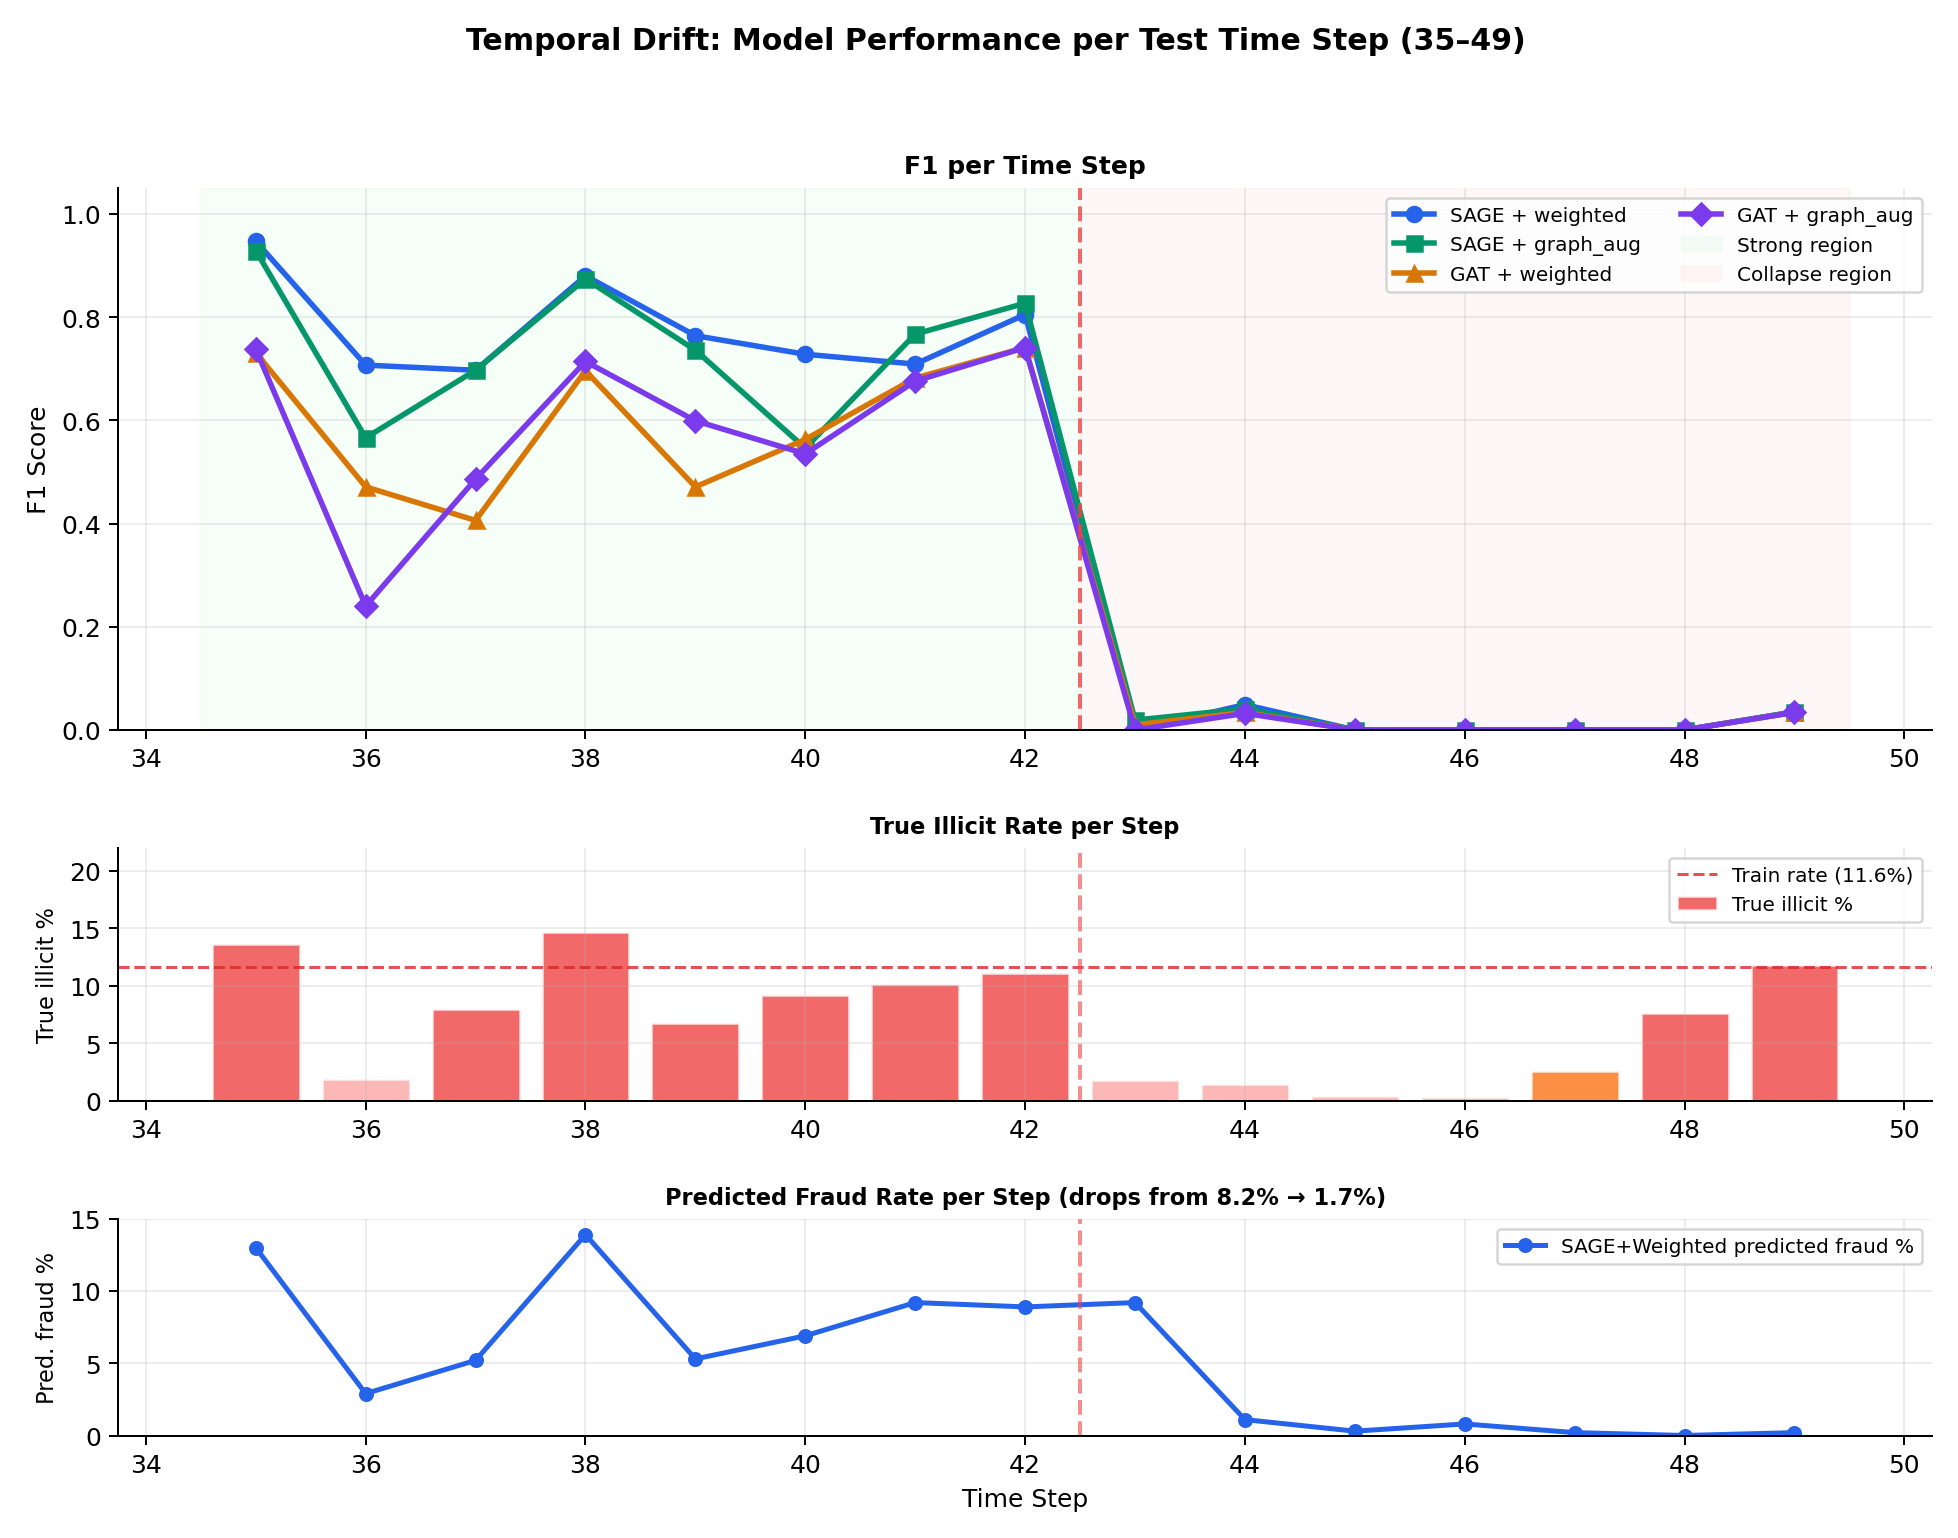
\includegraphics[width=\linewidth]{figures/fig2_temporal_drift.png}
\caption{Per-step F1 and illicit rate across the test window.  All
models collapse after step~42 as the illicit rate falls below 1\,\%.}
\label{fig:temporal}
\end{figure}

\subsection{Graph-Structure Ablation}

Table~\ref{tab:ablation} reports the edge-ablation results.  Shuffled
random edges outperform original transaction edges
(F1: 0.383 vs.\ 0.268), with Cohen's $d > 2$ and $p < 0.08$.  The
original graph is worse than random wiring.

\begin{table}[!htbp]
\centering
\caption{Graph-structure ablation (3 seeds).  Original edges degrade
performance below random rewiring.}
\label{tab:ablation}
\small
\begin{tabular}{lrr}
\toprule
\textbf{Edge condition} & \textbf{F1} & \textbf{AUC} \\
\midrule
Original edges & 0.268 & 0.811 \\
Shuffled edges & 0.383 & 0.839 \\
No edges (MLP) & 0.744 & 0.891 \\
\bottomrule
\end{tabular}
\end{table}

During training the fraud topology is stable and message passing
aggregates useful signals.  After the regime change, those edges
propagate stale priors that mislead the classifier.

\subsection{Hybrid Ensemble}

The concat hybrid---GNN embeddings concatenated with raw features,
classified by Random Forest---achieves F1\,=\,0.807
(Table~\ref{tab:hybrid}).  This recovers nearly all performance lost
by either component alone and confirms that graph-derived
representations carry complementary signal even when direct GNN
inference fails.

\begin{table}[!htbp]
\centering
\caption{Hybrid ensemble results.  Concat fusion nearly matches the
standalone RF while incorporating graph information.}
\label{tab:hybrid}
\small
\begin{tabular}{lr}
\toprule
\textbf{Configuration} & \textbf{F1} \\
\midrule
GNN embeddings only $\to$ RF & 0.311 \\
Raw features only $\to$ RF & 0.820 \\
Concat (GNN emb + raw) $\to$ RF & 0.807 \\
\bottomrule
\end{tabular}
\end{table}

The drop from 0.820 to 0.807 indicates that GNN embedding dimensions
introduce minor noise under shift, but the ensemble still outperforms
every standalone neural model.

\section{Analysis}

\subsection{Feature Attribution}

Random Forest feature importance shows 82.4\,\% of discriminative power
comes from local transaction features (the first 94 dimensions), with
17.6\,\% from aggregate neighbourhood statistics.  The MLP stays
competitive because the stable signal lives in local features that do
not depend on graph topology (Fig.~\ref{fig:features}).

\begin{figure}[!htbp]
\centering
\begin{minipage}[b]{0.48\linewidth}
  \centering
  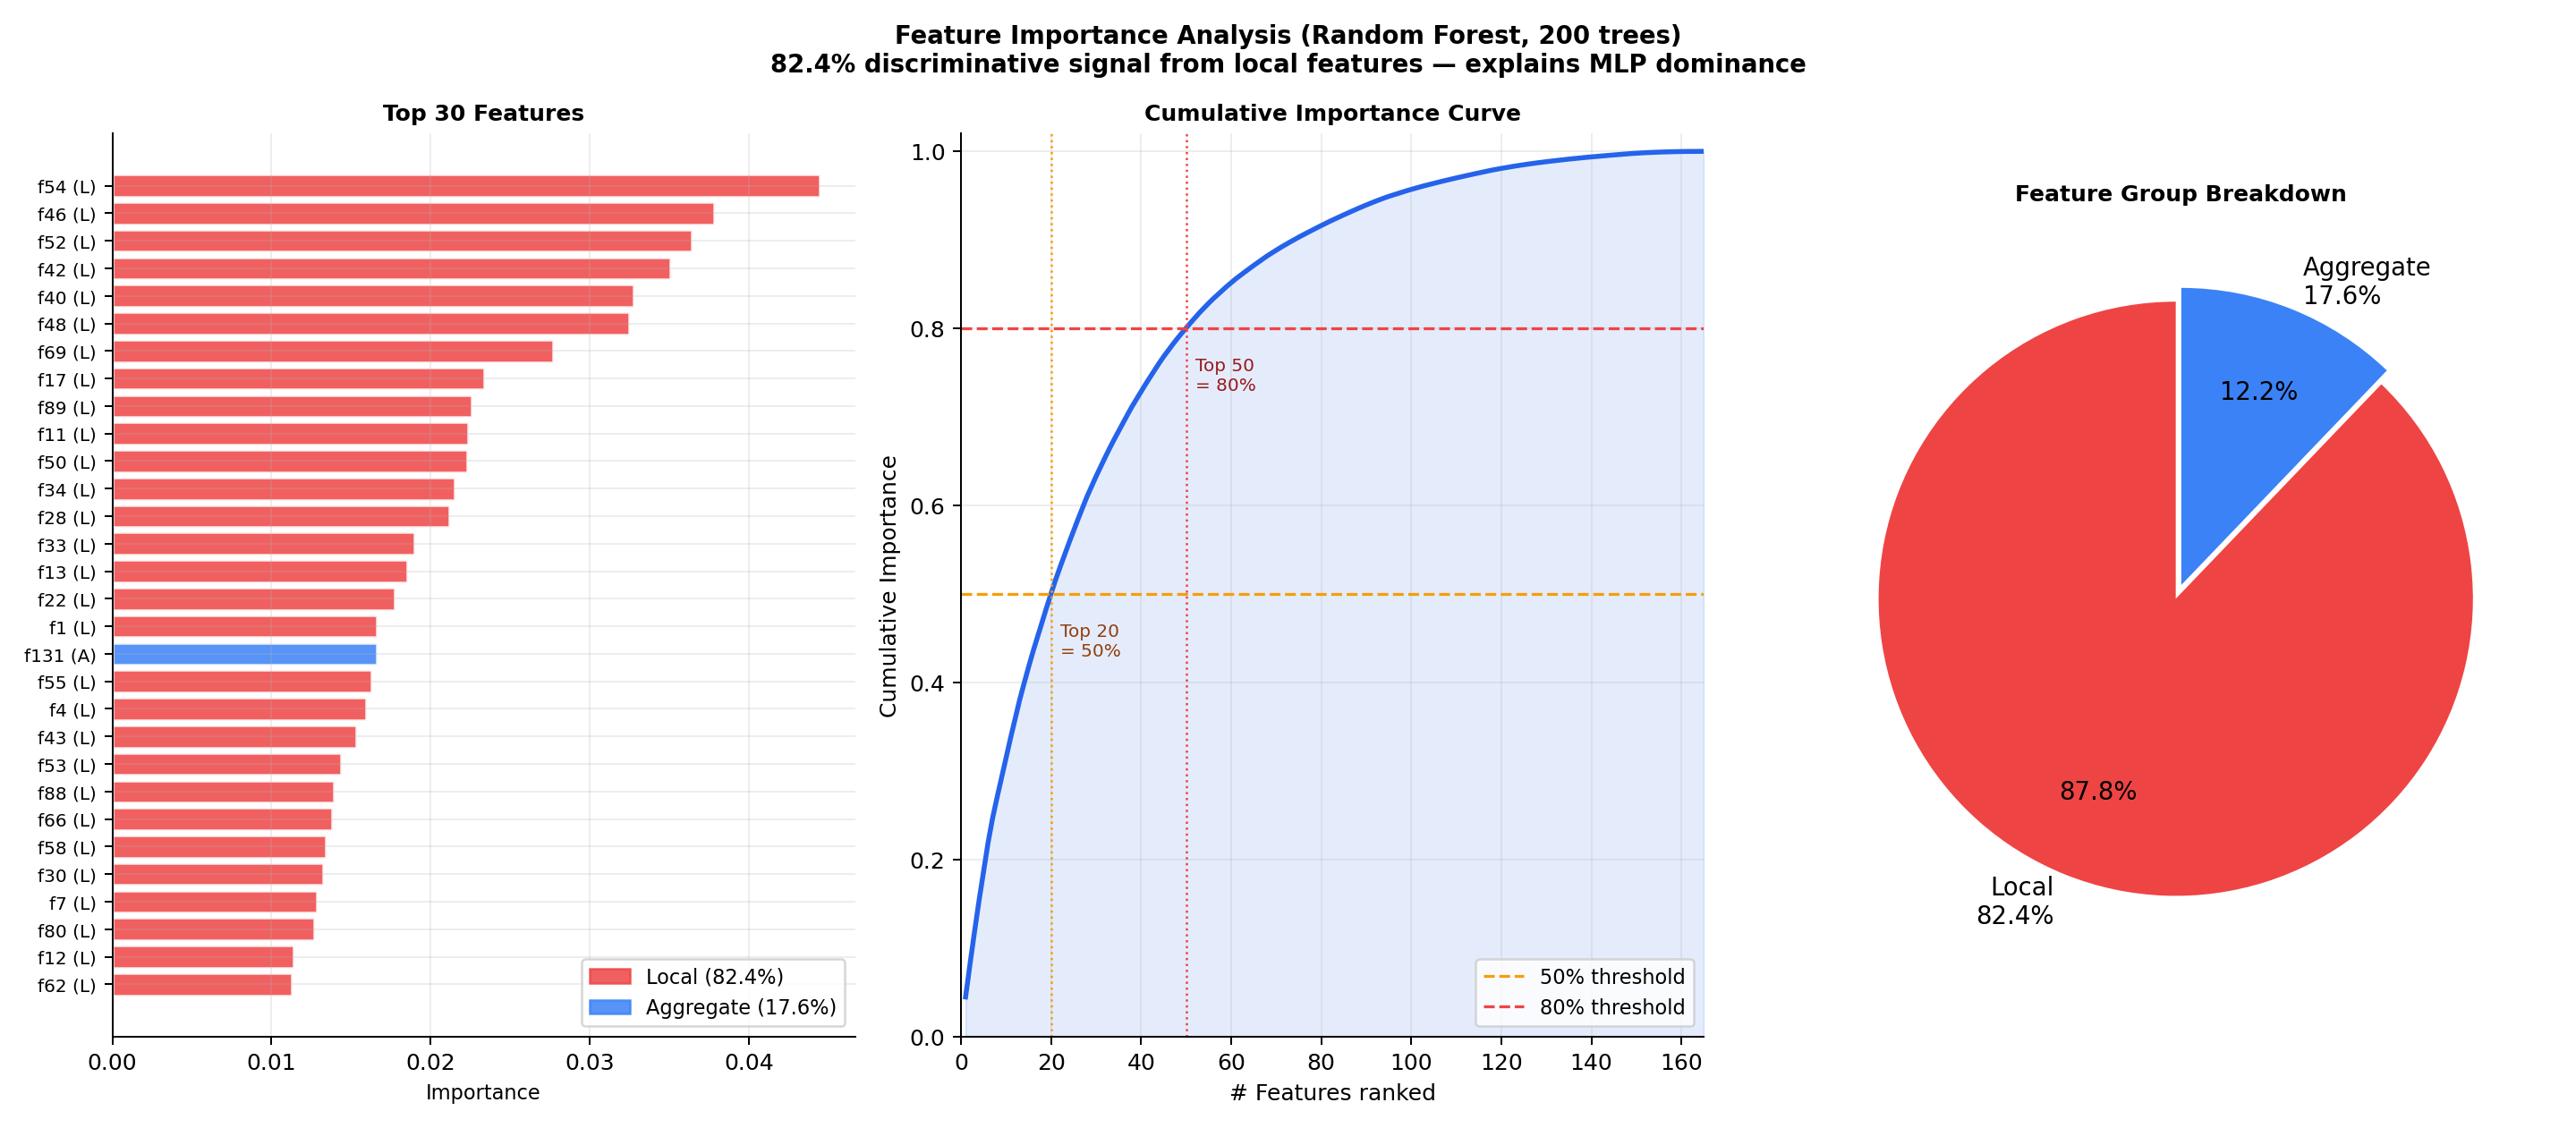
\includegraphics[width=\linewidth]{figures/fig4_feature_importance.png}\\[-0.2em]
  \footnotesize\textbf{(a)} Feature attribution.
\end{minipage}
\hfill
\begin{minipage}[b]{0.48\linewidth}
  \centering
  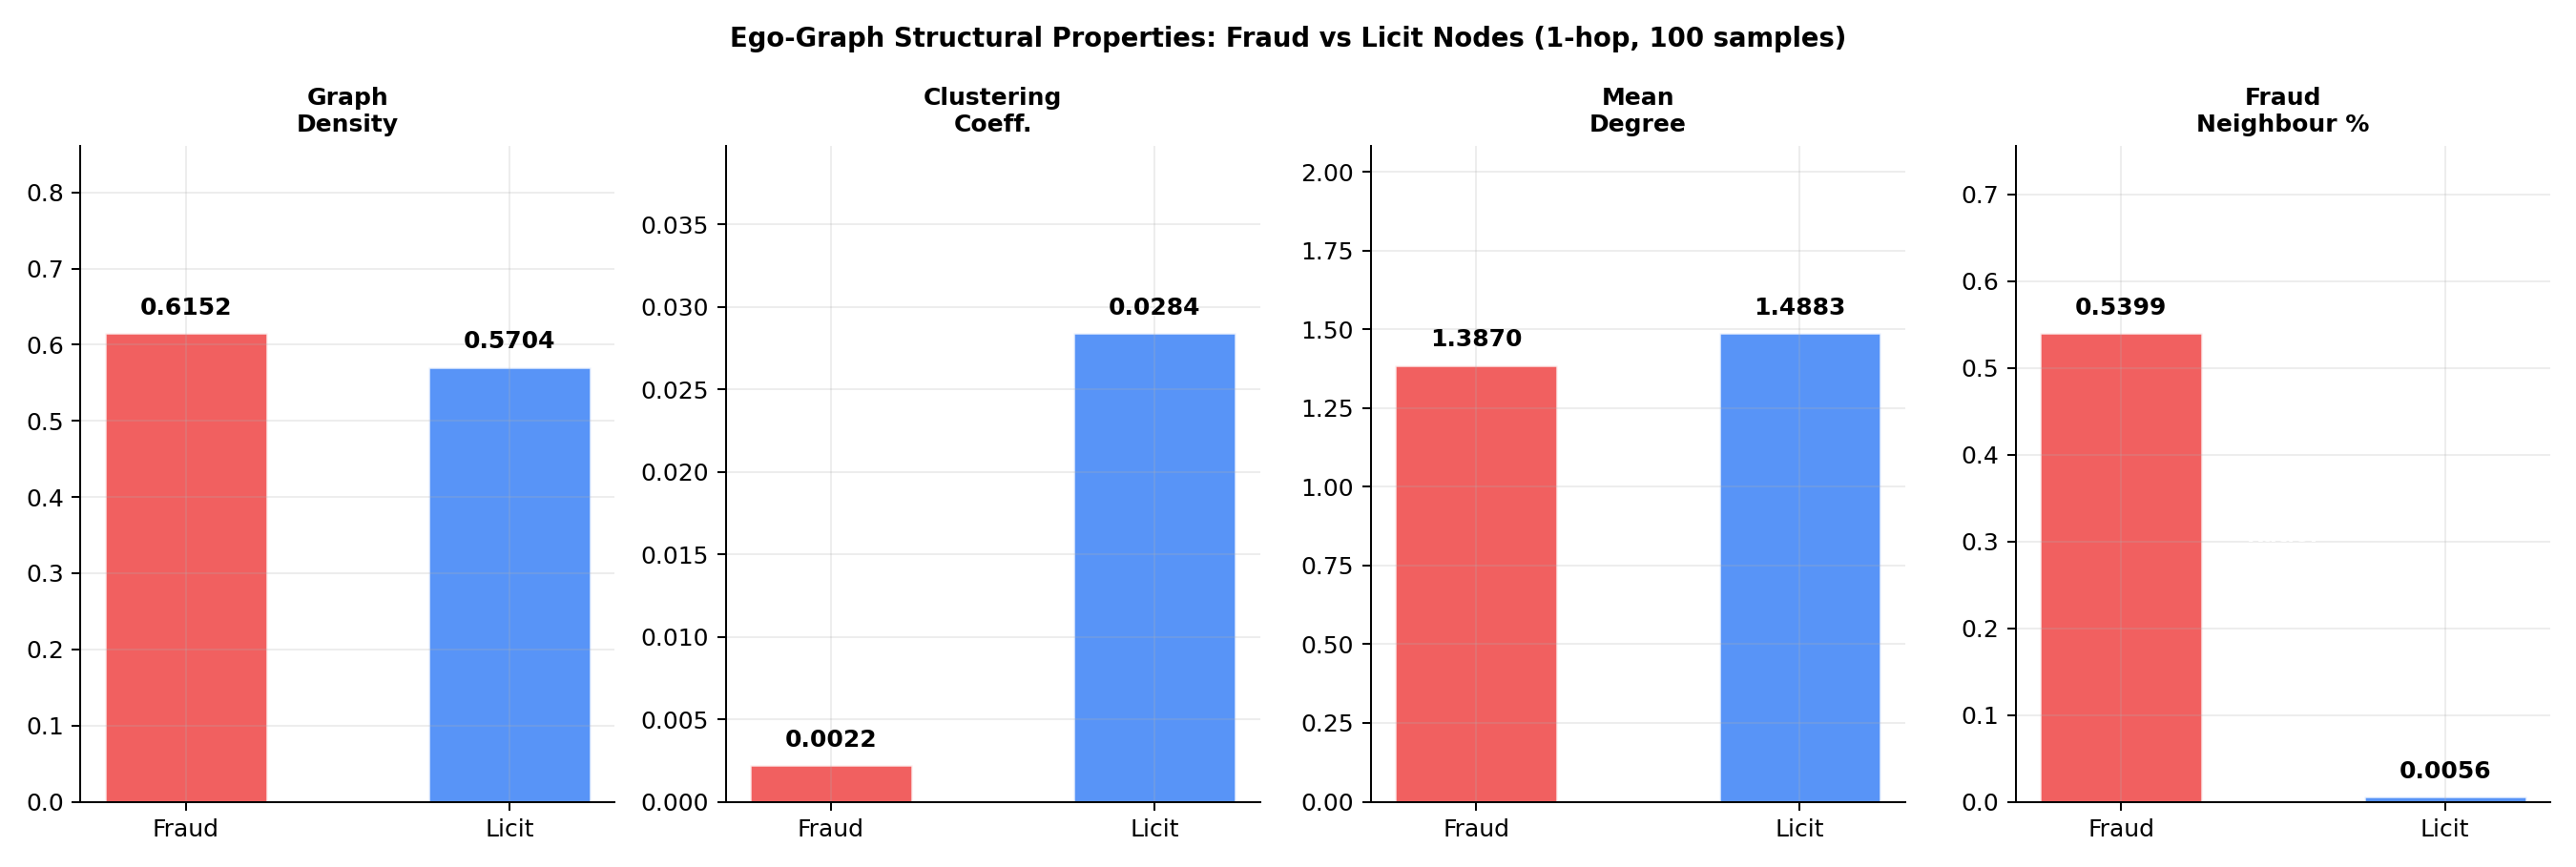
\includegraphics[width=\linewidth]{figures/fig5_community_structure.png}\\[-0.2em]
  \footnotesize\textbf{(b)} Community structure.
\end{minipage}
\caption{Local features dominate the stable signal (a), while
community structure exists but is temporally fragile (b).}
\label{fig:features}
\end{figure}

\subsection{Calibration}

Temperature scaling~\citep{guo2017calibration} yields $\Delta$F1\,=\,0
across all tested configurations (Table~\ref{tab:calibration}).  Fitted
temperatures fall between 0.92 and 1.04, indicating mild
overconfidence.  ECE barely moves: 0.284\,$\to$\,0.282 for SAGE
weighted, and SAGE graph augmentation actually worsens slightly
(0.173\,$\to$\,0.175).

\begin{table}[!htbp]
\centering
\caption{Temperature scaling results.  $\Delta$F1\,=\,0 across all
configurations; calibration cannot address temporal collapse.}
\label{tab:calibration}
\small
\begin{tabular}{lrrrr}
\toprule
\textbf{Model} & \textbf{$T^*$} & \textbf{ECE$_\text{pre}$}
  & \textbf{ECE$_\text{post}$} & \textbf{$\Delta$F1} \\
\midrule
SAGE weighted  & 1.041 & 0.284 & 0.282 & 0 \\
SAGE graph aug & 0.919 & 0.173 & 0.175 & 0 \\
GAT weighted   & 1.037 & 0.246 & 0.245 & 0 \\
GAT graph aug  & 1.027 & 0.266 & 0.266 & 0 \\
\bottomrule
\end{tabular}
\end{table}

Temperature scaling is rank-preserving: at a fixed threshold of 0.5, no
monotone transformation moves predictions across the boundary.  The
collapse is distributional, not calibration-related.

\subsection{Per-Step GNN Advantage}

Figure~\ref{fig:advantage} tracks per-step F1 difference between
GraphSAGE and MLP.  GraphSAGE holds a small advantage in steps 35--42
but the sign reverses in steps 43--49, marking where graph structure
turns from asset to liability.

\begin{figure}[!htbp]
\centering
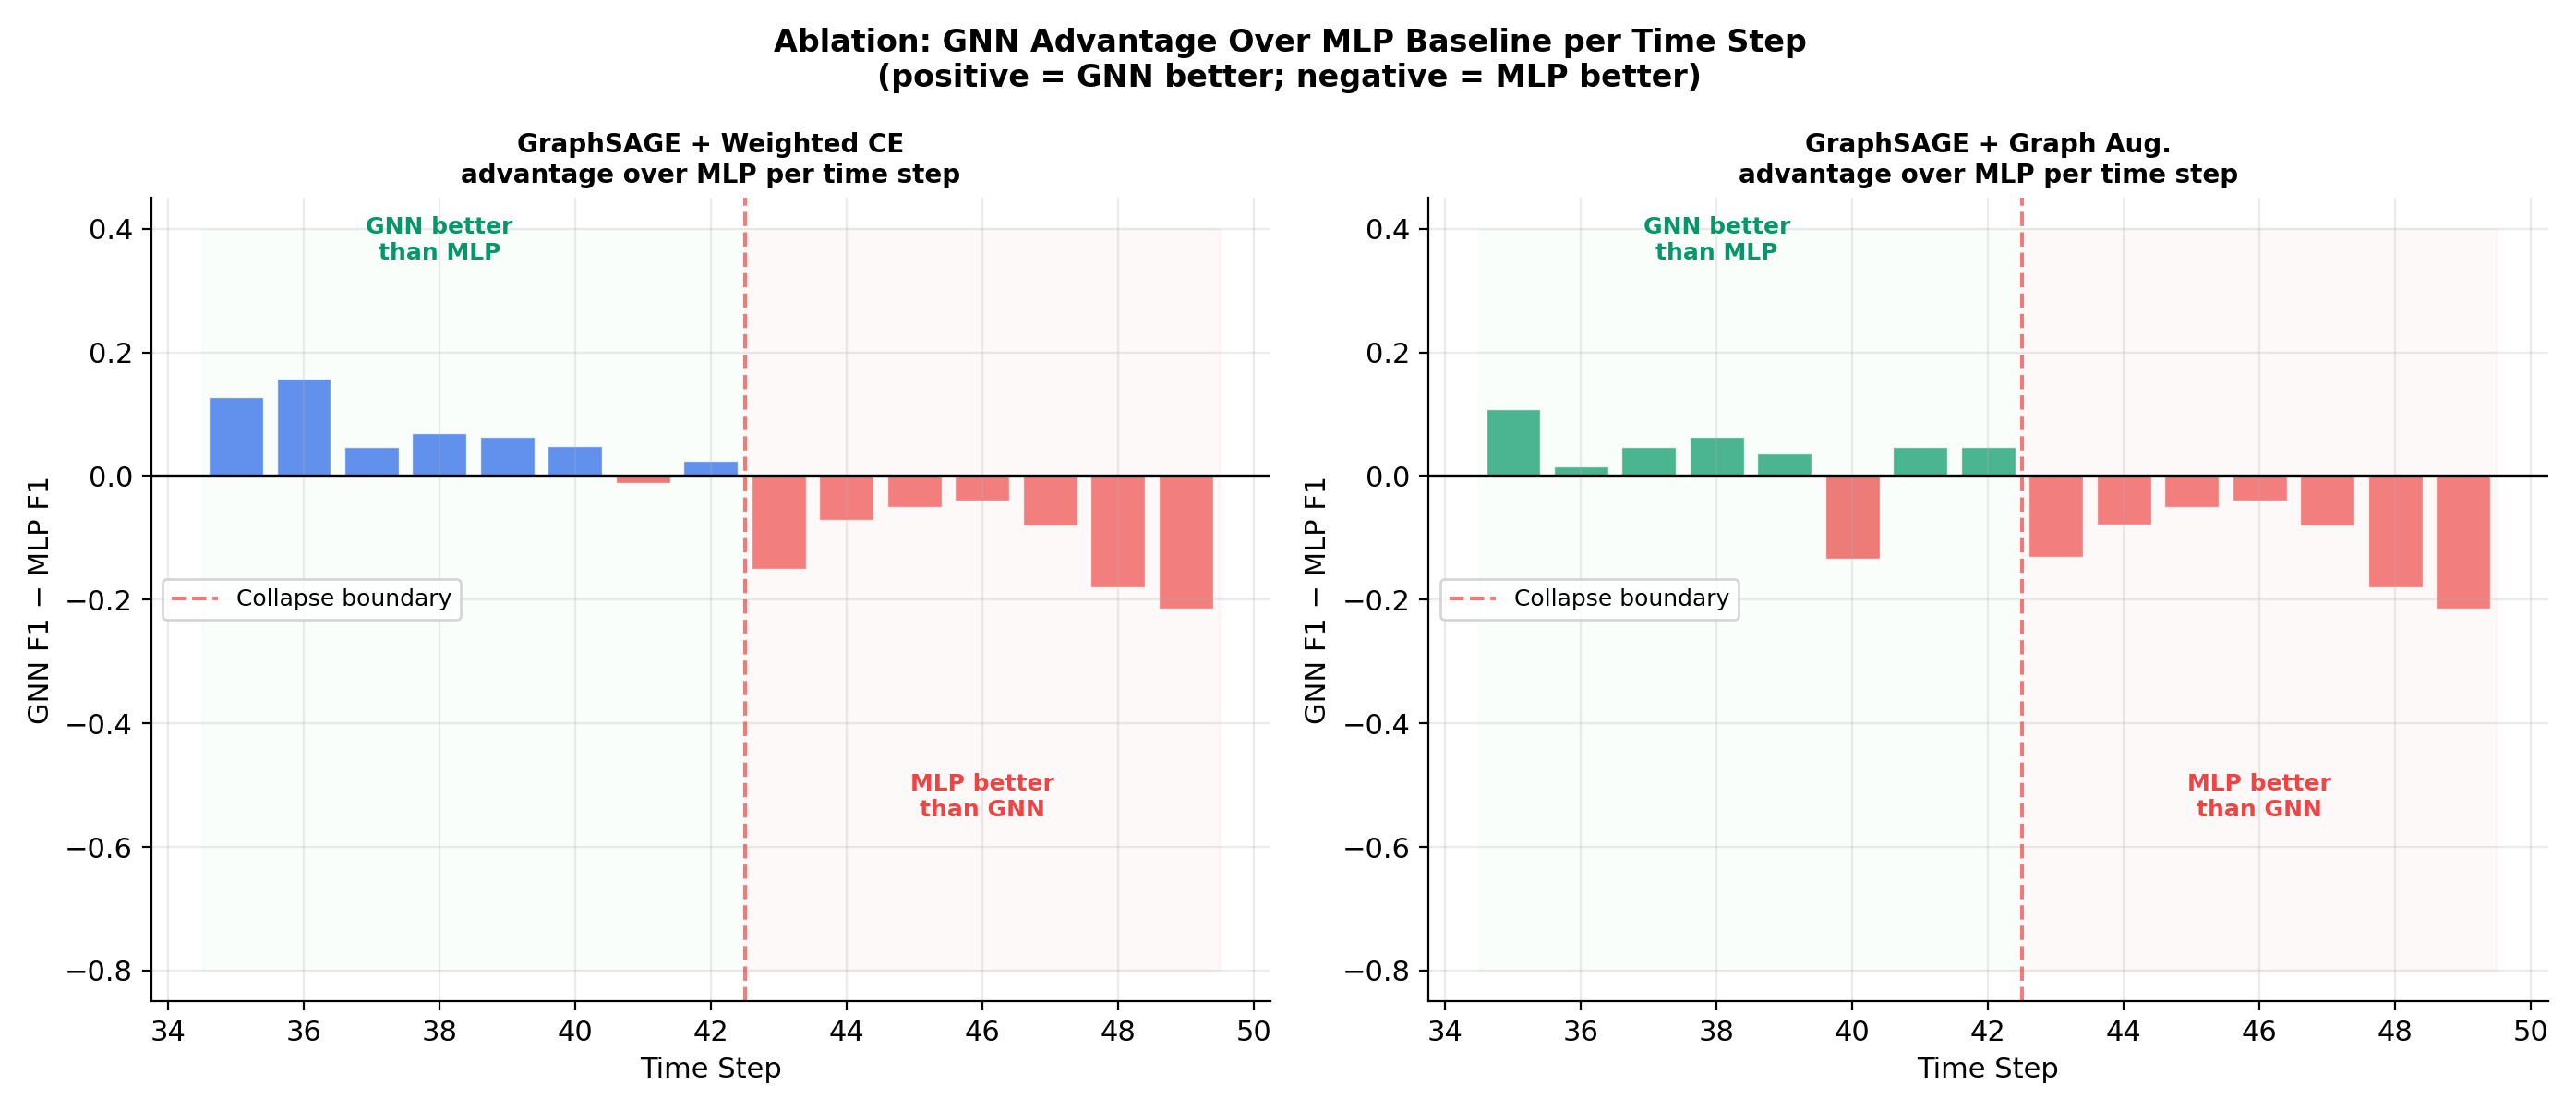
\includegraphics[width=\linewidth]{figures/fig16_ablation_advantage.png}
\caption{Per-step GraphSAGE advantage over MLP.  Positive values mean
the GNN is ahead; the sign reversal after step~42 marks where graph
structure becomes harmful.}
\label{fig:advantage}
\end{figure}

\section{Conclusion}

Three findings emerge from this benchmark.  First, under inductive
evaluation, no GNN matches a plain MLP on aggregate illicit-class F1,
and a Random Forest with no graph structure beats both
(F1\,=\,0.820 vs.\ 0.744 vs.\ 0.697).  Second, graph structure on the
original transaction edges actively degrades GNN performance: shuffled
edges improve F1 from 0.268 to 0.383, and removing edges entirely
(the MLP) improves it further.  Third, graph-derived representations
retain complementary value when fused with tabular features---the concat
hybrid achieves F1\,=\,0.807---but direct GNN inference on the raw
graph fails under temporal shift.

The practical implications are direct.  Periodic retraining is necessary
when the fraud rate moves this quickly; a static model trained at
11.6\,\% illicit cannot be expected to generalise to a 0.3\,\% regime.
Graph structure should be treated as a conditional asset rather than a
universal advantage.  Post-hoc calibration does not help ($\Delta$F1
and $\Delta$ECE both near zero).

The study uses a single dataset, and the inductive pipeline uses
RandomNodeLoader rather than full neighbour-sampling.  Future work
should test on additional temporal fraud benchmarks and explore adaptive
graph construction that responds to distributional shift.

\FloatBarrier

\bibliographystyle{splncs04}
\bibliography{references}

\end{document}
